\chapter{Analytical Calculations}

\section{Asymptotic behavior of the ordinary MSD}

The calculation of the MSD, both in the ordinary and in the aged case originally appeared in 
\cite{bothe} 
and are presented here again:

\subsection*{Calculation of $\gls{psi}_0(s)$}

All properties of the ordinary walk are derived from the waiting time density $\gls{psi}(t)$. The joint probability density of the displacement in a step and the duration of a step is given in the one dimensional case by
%
\begin{equation}
 \gls{psi}(x,t) = \frac{1}{2} \delta(|x| - ct^\nu ) \gls{psi}(t),
\end{equation}
%
so that the Fourier transform of this function in the $x$ variable reads
\begin{equation}
 \gls{psi}(k,t) = \gls{psi}(t) - \frac{k^2}{2} c^2 t^{2 \nu} \gls{psi}(t) + o(k^2). 
\end{equation}
%
Then the Laplace transform in $t$ should be performed.  Although the exact Laplace transform of $\gls{psi}(t)$ as given by Eq.(\ref{eqn:defPsiT}) is possible in quadratures, we are only interested in the asymptotic behavior, which can be found using the Tauberian theorem (\ref{eqn:generalTauberian}). The forms of the Laplace transform 
differ for different values of $\gamma$ and $\nu$. As explained above we are interested only in the lowest order terms of $s$-dependence. 

\subsubsection*{$ \gamma<1$}
For $0<\gamma <1$ the function $ \gls{psi}_0(s) = \gls{psi}(s)$ belongs to an integrable class, and its Laplace representation reads
\begin{equation}
 \gls{psi}_0(s) \simeq 1 + \gamma \Gamma(-\gamma) t_0^\gamma s^\gamma 
 = 1-\Gamma(1-\gamma) t_0^\gamma s^\gamma. \label{eqn:psi0GammaSmall}
\end{equation}
Keeping $t_0$ in all calculations and not putting it to unity is reasonable to be able to check the dimension of the ensuing results, especially in the aged case. 

\subsubsection*{$ \gamma>1$}
The Laplace transform of $\gls{psi}(t)$ now has an additional term, due to its first moment being finite:
\begin{equation}
\gls{psi}_{0}(s) \simeq 1 - \tau s - \Gamma(1-\gamma ) t_0^\gamma s^\gamma.
\label{eqn:psi0GammaBig}
\end{equation}  
Here $\tau$ is defined as 
\begin{equation}
 \tau = \frac{\gamma}{t_0} \int_0^\infty \frac{t dt}{(1+t/t_0)^{\gamma +1}} = 
 \frac{t_0}{\gamma-1} . \label{eq:tau}
\end{equation}

\subsection*{Calculation of $\gls{psi}_2(s)$}
The marginal second moment of the step distribution is given by  
\begin{align}
 \gls{psi}_2(t) = \int_{-\infty}^\infty x^2 \gls{psi}(x,t) dx = c^2 t^{2 \nu} \gls{psi}(t).
\end{align}
The expressions for $\gls{psi}_2(s)$ depend on whether $2 \nu < \gamma $ or $2 \nu > \gamma$:

\subsubsection*{$2\nu<\gamma$} 
In this first case the function $\gls{psi}_2(t)$ is integrable, $\int_0^\infty \gls{psi}_2(t) dt < \infty$, and the expansion 
of its Laplace transform starts from a constant:
\begin{equation}
 \gls{psi}_2(s) \simeq \gamma c^2 t_0^{2\nu}  \int_0^\infty \frac{x^{2\nu}}{(1+x)^{\gamma+1}} dx  + \gamma \Gamma(2\nu-\gamma) c^2t_0^\gamma s^{\gamma-2\nu} ,
\end{equation}
where the integral is given by a dimensionless constant:
\begin{equation}
 \int_0^\infty \frac{x^{2\nu}}{(1+x)^{\gamma+1}} dx = \mathrm{B}(2\nu+1,\gamma-2\nu), \label{eqn:I1}
\end{equation}
with $\mathrm{B}(a,b)$ being the Beta-function, which is defined as:
%
\begin{align}
\mathrm{B}(a,b) = \int_{0}^{1} x^{a-1}(1-x)^{b-1} dx = \frac{\Gamma(a)\Gamma(b)}{\Gamma(a+b)} .
\end{align}
%
With this $\gls{psi}_2(s)$ takes the form 
%
\begin{align}
\gls{psi}_2(s) \simeq \gamma c^2 t_0^{2\nu}  \mathrm{B}(2\nu+1,\gamma-2\nu)  + \gamma \Gamma(2\nu-\gamma) c^2t_0^\gamma s^{\gamma-2\nu} \label{eqn:psi2NuSmall} .
\end{align}

\subsubsection*{$2\nu>\gamma$} 
In the second case $\gls{psi}_2(t)$ is non-integrable, the integral $\int_0^\infty \gls{psi}_2(t) dt$ diverges, and the asymptotics of its Laplace transform read
\begin{align}
 \gls{psi}_2(s) \simeq \gamma \Gamma(2\nu-\gamma) c^2  t_0^\gamma s^{\gamma-2\nu}. \label{eqn:psi2NuBig}
\end{align}

\subsection*{Calculation of $\gls{comp}_0(s)$ and $\gls{comp}_2(s)$}

For complete steps our generalization does not differ from the original L\'evy walk and we can use the general result for $\gls{comp}(x,t)$ in the Fourier-Laplace domain Eq. (\ref{eqn:CFourierLaplace}):
%
\begin{align}
\gls{comp}(k,s) = \frac{1}{1 - \gls{psi}(k,s)}.
\end{align}
%
Expanding $\gls{comp}(k,s)$ for $s$ small and in the limit $k \to 0$ we find 
%
\begin{align}
\begin{split}
\gls{comp}(k,s)  &\simeq \frac{1}{1 - \gls{psi}(s) + (k^2/2) \gls{psi}_2(s) +o(k^2)}\\ &\simeq \frac{1}{1-\gls{psi}(s)} - \frac{k^2}{2}  \frac{\gls{psi}_2(s)}{[1-\gls{psi}(s)]^2} + o(k^2).
\end{split}
\end{align}
Therefore 
\begin{align}
\gls{comp}_0(s) =& \frac{1}{1-\gls{psi}(s)} , \\
\gls{comp}_2(s) =& \frac{\gls{psi}_2(s)}{[1-\gls{psi}(s)]^2} \;,
\end{align}
into which we now have to insert our results for $\gls{psi}_0$ and $\gls{psi}_2$:

\subsubsection{$\gamma<1$ and $2\nu<\gamma$ }
Here we find by using equations (\ref{eqn:psi0GammaSmall}) and (\ref{eqn:psi2NuSmall}) :
\begin{align}
 \gls{comp}_0(s) \simeq & \frac{1}{\Gamma(1-\gamma)} t_0^{-\gamma} s^{-\gamma}, \label{eq:Co}\\
 \gls{comp}_2(s) \simeq & \gamma   \frac{ \mathrm{B}(2\nu+1,\gamma-2\nu)}{\Gamma^2(1-\gamma)} c^2 t_0^{2\nu - 2\gamma} s^{-2 \gamma} .
\end{align}

\subsubsection{$\gamma<1 \text{ and } 2\nu>\gamma$: }
In this case we obtain for $\gls{comp}_2$:
\begin{equation}
  \gls{comp}_2(s) \simeq  \gamma   \frac{\Gamma(2\nu-\gamma)}{\Gamma^2(1-\gamma)} c^2 t_0^{-\gamma} s^{-2\nu-\gamma},
\end{equation}
while $\gls{comp}_0$ is the same as in Eq.(\ref{eq:Co}) as long as $\gamma<1$.

\subsubsection{$\gamma>1$ and  $2\nu<\gamma$}
Now the first moment of $\gls{psi}(t)$ is finite, therefore 
\begin{align}
 \gls{comp}_0(s) \simeq &  \frac{1}{\tau s}  \\
 \gls{comp}_2(s) \simeq & \gamma \mathrm{B}(2\nu+1,\gamma-2\nu) c^2 \frac{t_0^{2\nu}}{\tau^2}  s^{-2}
\end{align}


\subsubsection{$\gamma>1$ and $2\nu>\gamma$: }
Again $\gls{comp}_0(s)$ doesn't change, and for $\gls{comp}_2$ we obtain
\begin{equation}
\gls{comp}_2 \simeq  \gamma \Gamma(2\nu-\gamma)  c^2 \frac{t_0^\gamma}{\tau^2}   s^{\gamma-2\nu -2} .
\end{equation}

\subsection*{Calculation of  $\gls{rest}_0(s)$ and $\gls{rest}_2(s)$}
The function $\gls{rest}(x|t)$ gives the distribution of
the corresponding displacements conditioned on the fact that the total duration of a step is longer than $t$. In Eq. (\ref{eqn:defR}) we found the expression
%
\begin{equation}
 \gls{rest}(x|t) =  \int_t^\infty \frac{1}{2} \delta(|x| - c t^{\eta}t'^{\nu-\eta}) \gls{psi}(t') dt' \; .
\end{equation}
This is correctly normalized to the overall probability to stay within a single step for a time longer than $t$ 
\begin{equation}
 \int_{-\infty}^{\infty} \gls{rest}(x|t)  dx = \int_t^\infty \gls{psi}(t') dt'.
\end{equation}
Expanding the Fourier transform of $\gls{rest}(x,t)$ for small $k$,
\begin{align}
\gls{rest}(k|t) =& \int_{-\infty}^{\infty} dx \; e^{ikx} \int_t^\infty \frac{1}{2} \delta(|x| - c t^{\eta}t'^{\nu-\eta}) \gls{psi}(t') dt' \nonumber \\
=& \gls{rest}_0(t) - \frac{k^2}{2} \gls{rest}_2(t) + o(k^2), 
\end{align}
we find the marginal moments
\begin{align}
\gls{rest}_0(t) =& \frac{1}{(1+t/t_0)^{\gamma}} \\
\gls{rest}_2(t) =& \gamma c^2 \frac{1 }{t_0} t^{2\eta} \int_t^\infty \frac{t'^{2(\nu-\eta)}}{(1+t'/t_0)^{\gamma+1}} dt' \; , 
\end{align}
whose Laplace transforms depend on the relationship between $\gamma$, $\nu$ and $\eta$: 

\subsubsection{$\gamma<1 $ }
In this case $\gls{rest}_0$ is non-integrable and we find
\begin{equation}
  \gls{rest}_0(s) \simeq  \Gamma(1-\gamma) t_0^\gamma s^{\gamma-1}.
\end{equation}
For $\gls{rest}_2$  we can use the asymptotic form of $\gls{psi}(t)$ , since we are interested in large $t$:
\begin{equation}
\gls{rest}_2(t) \simeq \gamma c^2 t_0^\gamma t^{2\eta} \int_t^\infty \tau^{2(\nu-\eta)-1-\gamma}  d\tau   \; , 
\end{equation}
which is only finite for $\gamma > 2(\nu-\eta)$ and diverges otherwise, meaning that no MSD exists. In the rest of 
the paper we will concentrate on the case when the \gls{msd} is finite, where we find
\begin{equation}
\gls{rest}_{2}(t)  \simeq \gamma\frac{1} {\gamma - 2(\nu-\eta)} c^2 t_0^\gamma t^{2\nu -\gamma}  .
\end{equation}
Since this expression is always in the non-integrable class we obtain the following result by using the Tauberian theorem (\ref{eqn:tauberian}):
\begin{equation}
\gls{rest}_2(s) \simeq \gamma  \frac{ \Gamma(2\nu+1-\gamma)}{\gamma - 2(\nu-\eta)}c^2 t_0^\gamma s^{\gamma - 2\nu-1}.
\end{equation}

\subsubsection{$\gamma>1$ and $2\nu>\gamma-1$}
For $\gamma>1$ $\gls{rest}_0(t)$ becomes integrable, therefore its Laplace transform reads
\begin{equation}
 \gls{rest}_0 \simeq \tau + \Gamma(1-\gamma) t_0^\gamma s^{\gamma-1} .
\end{equation}
The function $\gls{rest}_2(t)$ is still non-integrable and therefore identical to the previous case.

\subsubsection{$\gamma>1$ and $2\nu<\gamma-1$}
In this case $\gls{rest}_0$ does not change but $\gls{rest}_2(s)$ is now integrable and therefore its transform behaves as
\begin{equation}
\gls{rest}_2(s) \simeq I^{\gls{rest}_2}_0 - \gamma \frac{\Gamma(2\nu+1-\gamma)}{2(\nu-\eta)-\gamma} c^2 t_0^\gamma s^{\gamma - 2\nu-1 } \; .
\end{equation}
We evaluate the definite integral $I^{\gls{rest}_2}_0$ by manipulating the area of integration:
\begin{align}
 I^{\gls{rest}_2}_0 =& c^2\int_0^\infty dt  t^{2\eta} \int_t^\infty dt' \gls{psi}(t') (t')^{2(\nu-\eta)} \\
  =& c^2\frac{1}{2\eta+1} \int_0^\infty \gls{psi}(t') t'^{2\nu+1} dt' \nonumber \\ 
 =& \gamma\frac{1}{2\eta+1} \int_0^\infty \frac{x^{2\nu+1}dx}{(1+x)^{\gamma+1}}c^2 t_0^{2\nu+1}  \nonumber \\
=& \gamma  \frac{\mathrm{B}(2\nu +2, \gamma - 2\nu -1)}{2\eta+1}  c^2 t_0^{2\nu+1} , 
\end{align}
meaning the $\gls{rest}_2$ is constant in the leading order. Therefore we find for $\gamma>1$ and $2\nu<\gamma-1$
%
\begin{align}
\gls{rest}_2 \simeq & \gamma \frac{\mathrm{B}(2\nu +2, \gamma - 2\nu -1)}{2\eta+1}  c^2 t_0^{2\nu+1}   -\gamma \frac{\Gamma(2\nu+1-\gamma)} {2(\nu-\eta)-\gamma} c^2 t_0^\gamma  s^{\gamma - 2\nu-1} .
\end{align}
%
The results so far are summarized in Table \ref{tab:Cr}.
%
\begin{center}
\begin{table}[htb]
 \begin{tabular}{||l|l|l||}
 \hline \hline
 \rule[-4mm]{0cm}{1cm} $\gamma<1$ & 
 $\gls{comp}_0(s) \simeq \frac{1}{\Gamma(1-\gamma)}t_0^{-\gamma} s^{-\gamma}$ & 
 $\gls{comp}_2(s) \simeq \left\{
\begin{array}{ll}
\gamma \frac{\mathrm{B}(2\nu+1,\gamma-2\nu)}{\Gamma^2(1-\gamma)} c^2 t_0^{2\nu - 2\gamma} s^{-2 \gamma} &\mbox{for } 2\nu < \gamma \\
 \gamma \frac{\Gamma(2\nu-\gamma)}{\Gamma^2(1-\gamma)} c^2 t_0^{-\gamma} s^{-2\nu-\gamma} &\mbox{for } 2\nu > \gamma
\end{array} \right. $ \\ \hline
\rule[-4mm]{0cm}{1cm}  $\gamma<1$ &$\gls{rest}_0(s) \simeq \Gamma(1-\gamma)t_0^\gamma s^{\gamma-1}$ & $\gls{rest}_2(s)  \simeq \gamma \frac{\Gamma(2\nu+1-\gamma)}{\gamma- 2(\nu-\eta)}c^2 t_0^\gamma s^{\gamma-1-2\nu}$ \\ \hline
\rule[-4mm]{0cm}{1cm}   $\gamma>1$ & $\gls{comp}_0(s) \simeq   \frac{1}{\tau s}$ & 
 $\gls{comp}_2(s) \simeq \left\{ \begin{array}{ll}
 \gamma \mathrm{B}(2\nu+1,\gamma-2\nu)c^2 \frac{t_0^{2\nu}}{\tau^2}  s^{-2} & \mbox{for } 2\nu < \gamma \\
\gamma \Gamma(2\nu-\gamma)c^2\frac{t_0^\gamma}{\tau^2} s^{\gamma-2\nu -2}  & \mbox{for }  2\nu > \gamma
\end{array} \right. $\\ \hline
\rule[-4mm]{0cm}{1cm} $\gamma>1$ &$\gls{rest}_0(s) \simeq\ \tau$ 
 & $\gls{rest}_2(s) \simeq \left\{ \begin{array}{ll}
\gamma\frac{\mathrm{B}(2\nu +2, \gamma - 2\nu -1)}{2\eta+1}  c^2 t_0^{2\nu+1}  & \mbox{for } 2\nu < \gamma -1 \\
\gamma \frac{\Gamma(2\nu+1-\gamma)}{\gamma - 2(\nu-\eta)}  c^2 t_0^\gamma   s^{\gamma - 2\nu-1}& \mbox{for } 2\nu > \gamma -1 
\end{array} \right.$ \\ \hline \hline
\end{tabular}
\caption{Leading terms of the marginal moments of $C$  and $r$ in the Laplace domain for different parameter ranges. 
\label{tab:Cr}}
\end{table}
\end{center}



\subsection*{Mean squared displacement}
With these results we can now compute the MSD via the formula
\begin{equation}
\langle x^2(s) \rangle = \gls{comp}_0(s) \gls{rest}_2(s) + \gls{comp}_2(s) \gls{rest}_0(s) \; .
\end{equation}

\subsubsection{$\gamma<1$ and $2\nu < \gamma$: }
In the case  $2\nu < \gamma $ we have
\begin{equation}
\begin{split}
\langle x^2(s) \rangle  \simeq   \gamma  & \left[\frac{\Gamma(2\nu +1-\gamma)}{\Gamma(1-\gamma)(\gamma - 2(\nu-\eta))}c^2 s^{-2\nu -1} \right. \\
& \left. + \frac{\mathrm{B}(2\nu+1,\gamma-2\nu)}{\Gamma(1-\gamma)}c^2 t_0^{2\nu-\gamma} s^{-\gamma -1} \right] , 
\end{split}
\end{equation}
which translates to
\begin{equation}
\begin{split}
 \langle x^2(t) \rangle \simeq \gamma  & \left[\frac{\Gamma(2\nu +1-\gamma)}{\Gamma(1-\gamma)(\gamma-2(\nu-\eta))\Gamma(2\nu + 1)} c^2 t^{2\nu} \right. \\ 
 & \left.  + \frac{\mathrm{B}(2\nu+1,\gamma-2\nu)}{\Gamma(1-\gamma)\Gamma(1+\gamma)} c^2 t_0^{2\nu-\gamma} t^{\gamma} \right].
 \end{split}
\end{equation}
This is dominated by the second term since $2\nu < \gamma$, leading to  $\langle x^2(t) \rangle \propto t^\gamma$ in this case. 

%It follows that for $\gamma < 1$ and $2\nu < \gamma$ the behavior of the walk merges with the one of a CTRW
%with a fixed step length.

\subsubsection{$\gamma<1$ and  $2\nu > \gamma$ }
In this parameter regime we obtain
\begin{align}
 \langle x^2(s) \rangle \simeq & \gamma c^2 s^{-2\nu-1}  \left[\frac{\Gamma(2\nu+1-\gamma)}{\Gamma(1-\gamma)(\gamma - 2(\nu-\eta))} +  \frac{\Gamma(2\nu-\gamma)}{\Gamma(1-\gamma)} \right]  \nonumber \\
 = & \gamma  \frac{\Gamma(2\nu -\gamma)}{\Gamma(1-\gamma)} \frac{2\eta }{\gamma - 2(\nu-\eta)}c^2  s^{-2\nu-1} ,
\end{align}
therefore we find in the time domain
\begin{equation}
 \langle x^2(t) \rangle \simeq \gamma \frac{\Gamma(2\nu -\gamma)} {\Gamma(2\nu+1) \Gamma(1-\gamma)} \frac{2\eta}{2(\nu-\eta)-\gamma}  c^2  t^{2\nu} .
\end{equation}

\subsubsection{$\gamma>1$ and $2\nu < \gamma-1$}
In this case the MSD reads
\begin{align}
\langle x^2(s) \rangle =& \gls{comp}_0(s) \gls{rest}_2(s) + \gls{comp}_2(s)  \gls{rest}_0(s) \nonumber \\
 \simeq & \gamma \frac{\mathrm{B}(2\nu +2, \gamma - 2\nu -1)}{2\eta+1} c^2 \frac{t_0^{2\nu+1}}{\tau}\frac{1} {s}   + \gamma \mathrm{B}(2\nu+1,\gamma-2\nu) c^2 \frac{t_0^{2\nu}}{\tau}  s^{-2} \nonumber ,
\end{align}
which is dominated by the second term. Therefore we find in the time domain to leading order:
\begin{equation}
\langle x^2(t) \rangle \simeq \gamma \mathrm{B}(2\nu+1,\gamma-2\nu) c^2 \frac{ t_0^{2\nu}}{\tau}  t.
\end{equation}

\subsubsection{$\gamma>1 \text{ and }  \gamma-1 <2\nu < \gamma$}
Compared to the previous case only $\gls{rest}_2$ changes, therefore
\begin{align}
\langle x^2(s) \rangle &\simeq & \gamma \frac{\Gamma(2\nu+1-\gamma)}{\gamma - 2(\nu-\eta)} c^2\frac{t_0^{\gamma}}{\tau}  s^{\gamma-2-2\nu}  + \gamma \mathrm{B}(2\nu+1,\gamma-2\nu) c^2\frac{t_0^{2\nu}}{\tau}  s^{-2} .
\end{align}
Since $\gamma-2\nu>0$ the term quadratic in $s$ is again dominant, and the asymptotic behavior in the time domain is identical to the previous case:
\begin{equation}
\langle x^2(t) \rangle \simeq   \gamma \mathrm{B}(2\nu+1,\gamma-2\nu) c^2
\frac{t_0^{2\nu}}{\tau}  t.
\end{equation}

\subsubsection{$\gamma>1$ and $2\nu > \gamma$}
Now $\gls{comp}_2$ is different, giving us 

\begin{align}
\langle x^2(s) \rangle \simeq & \gamma \frac{\Gamma(2\nu+1-\gamma)}{\gamma - 2(\nu-\eta)} c^2 \frac{t_0^{\gamma}}{\tau}  s^{\gamma-2\nu-2} + \gamma \Gamma(2\nu-\gamma) c^2\frac {t_0^{\gamma}}{\tau}  s^{\gamma-2\nu-2}. 
\end{align}
This leads to the time dependence 
\begin{equation}
\langle x^2(t) \rangle \simeq \gamma   \frac{2 \eta }{\gamma - 2(\nu-\eta) } \frac{\Gamma(2\nu-\gamma)}{\Gamma(2\nu + 2-\gamma)} c^2  \frac{t_0^{\gamma}}{\tau } t^{2\nu+1-\gamma}.
\end{equation}

The results for the ordinary walk under the assumption that the convergence condition $\gamma > 2(\nu-\eta)$ is satisfied can be summarized as follows: 
\begin{equation}
\langle x^2(t) \rangle \propto \left\{
  \begin{array}{lll}
  t^{\gamma} & \mathrm{for} & \gamma < 1, \; 2\nu < \gamma \\
t^{2\nu} & \mathrm{for} & \gamma < 1, \; 2\nu > \gamma \\
t & \mathrm{for} & \gamma > 1, \; 2\nu < \gamma \\
t^{2\nu+1- \gamma  } &\mathrm{for} &  \gamma > 1, \;2\nu > \gamma .
  \end{array}
  \right.
\label{balpoint}
\end{equation}
Thus, in the whole domain of $\gamma$ there are four regimes with crossovers at $\gamma = 1$ and at $2\nu = \gamma$:
\begin{itemize}
 \item For $2\nu < \gamma$ one has $\langle x^2(t) \rangle \propto t^{\gamma}$ for $\gamma <1$ crossing over to a faster growth $\langle x^2(t) \rangle \propto t$ for $\gamma > 1$
 \item For $2\nu > \gamma$ one has universally $\langle x^2(t) \rangle \propto t^{2\nu}$ for $\gamma <1$ crossing over to a slower growth $\langle x^2(t) \rangle \propto t^{2\nu+1-\gamma}$ for $\gamma > 1$.
\end{itemize}


\section{Aged walk: general expressions }
\label{Sec:Aged}

We now consider the functions $F$ and $s$ which are specific to aged walks. The general expression for $F$ reads: 
\begin{align}
 F(x,t|t_a)= \int_0^{t_a} dt' & \gls{psi}(t_a+t-t') k(t') \\
& \times \frac{1}{2}\delta \left\{\abs{x}
-c[(t_a+t-t')^\nu-(t_a+t-t')^{\nu-\eta} (t_a-t')^\eta]\right\} , \nonumber
\end{align}
where $k(t)=\gls{comp}_{0}(t)$ is the time-dependent rate of steps. Note that the argument of the $\delta$-function is shifted, 
due to the fact that the distance from the origin $x$ is set to zero at the start of the measurement. The marginal density of $F(x,t|t_a)$ is
\begin{align}
\gls{first}_0(t|t_a) =& \int F(x,t|t_a) dx =\int_0^{t_a} \gls{psi}(t_a+t-t') k(t') dt' \nonumber \\
 =& \gls{psi}_1(t|t_a),
\end{align}
where $\gls{psi}_1(t|t_a)$ is the forward waiting time PDF known from the theory of \gls{ctrw} as discussed in Sec. (\ref{sec:forwardWaiting}). The marginal second moment of $F$ reads:
\begin{align}
\gls{first}_2(t|t_a) = \int_0^{t_a} dt' & c^2 \gls{psi}(t_a+t-t') k(t')  \label{eqn:F2} \\ 
& \times [(t_a+t-t')^\nu-(t_a+t-t')^{\nu-\eta} (t_a-t')^\eta]^2 . \nonumber
\end{align}
Additionally we have to consider the term $s(x|t,t_a)$, which describes the case that both the aging time and the observation time belong to the same step:
\begin{align}
 s(x|t,t_a) = \int_0^{t_a} dt' & k(t') \int^{\infty}_{t_a+t-t'} dt'' \gls{psi}(t'')  \\
& \times \frac{1}{2} \delta \left\{\abs{x}-c[(t'')^{\nu-\eta}(t_a+t-t')^\eta-(t'')^{\nu-\eta}(t_a-t')^{\eta}]\right\} , \nonumber 
\end{align}
where the inner integral gives the probability that no change point took place during the time interval between $t'$ and $t_a+t$. The zeroth order of this function,
\begin{equation}
 s_0(t,t_a) = \int_0^{t_a} \gls{surv}(t_a+t-t') k(t') dt'  ,
\end{equation}
where $\gls{surv}(t) = \int_t^\infty \gls{psi}(t') dt'$ is the survival probability,
is not necessary for what follows, and will not be calculated. \\
The second moment is given by
\begin{align}
\begin{split}
 s_2(t,t_a) =c^2 \int_0^{t_a} & k(t') \int^{\infty}_{t_a+t-t'}  \gls{psi}(t'')  \\ 
& \;\; \times [(t'')^{\nu-\eta}(t_a+t-t')^\eta-(t'')^{\nu-\eta}(t_a-t')^{\eta}]^2   dt'' dt'  \label{eqn:s2} .
\end{split}
\end{align}
We note that the form of the integrals involved in $\gls{first}_2$ and $s_2$ is very similar. 
In the following calculation we differentiate between two time regimes: The case of short aging times $t>>t_a>> t_0$ and the case of long aging times $t_a>>t>>t_0$, 
which will be discussed separately in the two following sections. 

\section{Aged walk: short aging times $t>> t_a$}

\subsection*{Calculation of $\gls{first}_0$ and $\gls{first}_2$}

We are interested in the Laplace transforms of the marginal moments of $\gls{first}_0$ and $\gls{first}_2$. Since both of them depend on $k(t)=\gls{comp}_0(t)$ 
whose form we found to be dependent on whether $\gamma<1$ or $\gamma>1$, so we have to distinguish between these cases:

\subsubsection{$\gamma<1$}
The function $\gls{first}_0(t|t_a)$ is equal to the forward waiting time PDF $\gls{psi}_1(t|t_a)$. For $\gamma<1$ we can use the result from Eq. (\ref{eqn:forwardWaiting})
\begin{equation}
 \gls{first}_0(t|t_a) = \gls{psi}_1(t|t_a) = \frac{\sin \pi \gamma}{\pi} \left( \frac{t_a}{t}\right)^\gamma \frac{1}{t+t_a}. \label{eqn:psi1}
\end{equation}
The expression is normalized to unity, and therefore in the Laplace domain the leading term in $\gls{first}_0$ will be 1. 

For $t>>t_a$ the expression in the square brackets in Eq.(\ref{eqn:F2}) can be approximated by $t^{2\nu}$ (since $\nu > 0$) and for $\gls{first}_2$ we find in this limit
\begin{equation}
 \gls{first}_2(t|t_a) \simeq  c^2 t^{2\nu} \int_0^{t_a} \gls{psi}(t_a+t-t') k(t') dt'.
\end{equation}
The integral can again be expressed through the forward waiting time $\gls{psi}_1(t|t_a)$. We take the asymptotics of $\gls{psi}_1$ for $t$ large, so that 
\begin{equation}
\gls{first}_2(t|t_a) \simeq \frac{\sin \pi \gamma}{\pi} c^2  t_a^\gamma t^{2\nu-\gamma -1}  .  
\end{equation}
Here again two situations arise depending on the integrability: 

\subsubsection{$\gamma <1$ and  $2 \nu > \gamma$}
In this case $\gls{first}_2$ is non-integrable, so that in the Laplace domain
\begin{equation}
 \gls{first}_2(s|t_a) \simeq \Gamma(2\nu-\gamma) \frac{\sin \pi \gamma}{\pi} c^2 t_a^\gamma s^{\gamma - 2\nu}.
\end{equation}

\subsubsection{$\gamma <1$  and $2\nu < \gamma $} 
Now $\gls{first}_2$ is integrable, and the lowest order in its Laplace transform tends to a constant:
\begin{equation}
 \gls{first}_2(s|t_a) \simeq \frac{\sin \pi \gamma}{\pi}  c^2 t_a^\gamma \int_0^\infty \frac{ t^{2\nu-\gamma}}{t+t_a} dt.
\end{equation}
The corresponding integral is given by
\begin{equation}
 \int_0^\infty \frac{t^{2\nu-\gamma}}{t+t_a} dt = \frac{\pi }{\sin (\pi(2\nu +1- \gamma))}t_a^{2\nu - \gamma} ,
\end{equation}
see Eq.(2.2.5.25) of Ref. \cite{BryPr}, so that
\begin{equation}
 \gls{first}_2(s|t_a) \simeq   \frac{\sin \pi \gamma}{\sin (\pi(2\nu +1- \gamma))}c^2 t_a^{2\nu}.
\end{equation}

\subsubsection{$\gamma > 1$}
Now we consider the case $\gamma > 1$. From the previous section we know that $\gls{comp}_0(s)=\frac{1}{\tau s}$, therefore
\begin{equation}
k(t) =\gls{comp}_0(t)= \frac{1}{\tau} . \label{eqn:kGammaLarge}
\end{equation}
With this we can rewrite $\gls{first}_0$ as 
\begin{equation}
 \gls{first}_0(t|t_a) = \frac{1}{\tau} \int_0^{t_a} \gls{psi}(t+y)dy.
\end{equation}
For $t \to \infty$ the integral decays as $t^{-\gamma-1}$ and therefore is of integrable type. To find its lowest order (constant) term of the Laplace transform we note that
\begin{align}
 \gls{first}_0(s|t_a) \simeq & \frac{1}{\tau} \int_0^\infty dt \int_0^{t_a} \gls{psi}(t+y)dy \\
 =& \frac{1}{\tau} \int_0^{t_a} dy \int_0^\infty dt \gls{psi}(t+y)  \\
 =& \frac{1}{\tau} \int_0^{t_a} dy \int_y^\infty dt \gls{psi}(t) \\
 =& \frac{1}{\tau} \int^{t_a}_0 \gls{surv}(y) dy,
\end{align}
where $\Psi(t) = \int_t^\infty dt' \gls{psi}(t')$ is the so-called survival probability which is normalized to $\int_0^\infty \gls{surv}(t') dt' = \tau$. Since $t_a \gg t_0$ the whole integral therefore tends to $\tau$. 

The term $\gls{first}_2$ for $t \gg t_a$ can again be 
evaluated by approximating the expression in square brackets in Eq.(\ref{eqn:F2}) by $t^\nu$: 
\begin{align}
 \gls{first}_2(t|t_a) \simeq & c^2  \frac{1}{\tau} t^{2\nu} \int_0^{t_a} \gls{psi}(t+y)dy \\
 =& c^2 \frac{ t_0^\gamma }{\tau} [(t+t_0)^{-\gamma}-(t+t_a+t_0)^{-\gamma}]t^{2\nu}. 
\label{F2lagrer1}
\end{align}
Since the power law asymptotics of the expression in square brackets are $t^{-\gamma -1}$ the whole expression
\begin{equation}
 \gls{first}_2(t|t_a) \simeq \gamma c^2  \frac{t_0^\gamma }{\tau}t_a t^{2\nu-\gamma -1}
\end{equation}
is of the non-integrable type for $2\nu > \gamma$ and of integrable type for $2 \nu < \gamma$.

\subsubsection{$\gamma>1$ and $2\nu > \gamma$} 
In this first case $\gls{first}_2(t|t_a)$ is non-integrable, therefore the Laplace transform is 
\begin{equation}
 \gls{first}_2(s|t_a) \simeq \gamma\Gamma (2\nu-\gamma) c^2\frac{t_0^\gamma}{\tau}t_a s^{\gamma - 2\nu}.
\end{equation}

\subsubsection{$\gamma>1$ and $2\nu < \gamma$}
In the second case the Laplace transform of the expression tends to a constant. To evaluate this we put down 
\begin{equation}
 \gls{first}_2 \simeq  \gamma c^2 \frac{t_0^\gamma}{\tau} \int_0^\infty dt \; t^{2\nu} \int_0^{t_a} \frac{1}{(t+t_0+y)^{\gamma+1}} dy \; ,
\end{equation}
and interchange the sequence of integrations:
\begin{align}
 \gls{first}_2 =& \gamma c^2 \frac{ t_0^\gamma}{\tau} \int_0^{t_a} dy \int_0^\infty \frac{t^{2\nu}}{(t+t_0+y)^{\gamma+1}} dt \nonumber \\
 =& \gamma \mathrm{B}(2\nu+1,\gamma - 2\nu) c^2 \frac{ t_0^\gamma}{\tau}  \int_0^{t_a} (t_0+y)^{2\nu -\gamma} dy \nonumber \\
 =& \gamma  \frac{\mathrm{B}(2\nu+1,\gamma - 2\nu) }{2 \nu +1- \gamma } c^2 \frac{t_0^\gamma}{\tau} [(t_0+t_a)^{2\nu +1- \gamma }-t_0^{2\nu+1 - \gamma }]. \nonumber
\end{align}
%
(in the transition to the second line the Eq.(2.2.5.24) of Ref. 
\cite{BryPr} 
is used). The corresponding expression is dominated by the first or by the second term in the square 
brackets, depending on whether $2\nu > \gamma -1$ or $2\nu < \gamma -1$. \\
We summarize our results for $\gamma > 1$ in the following formula:
\begin{equation}
 \gls{first}_2 = \left\{
 \begin{array}{ll}
   \gamma \frac{\mathrm{B}(2\nu+1,\gamma - 2\nu)}{ \gamma -1 - 2 \nu} c^2 \frac{  t_0^{2\nu +1}}{\tau}  & \mbox{for } 2\nu < \gamma -1 \\
  \gamma \frac{\mathrm{B}(2\nu+1,\gamma - 2\nu)}{2 \nu - \gamma +1} c^2 \frac{ t_0^\gamma}{\tau} t_a^{2\nu +1- \gamma }  & \mbox{for } \gamma-1 < 2\nu < \gamma \\ 
 \gamma \Gamma(2\nu-\gamma) c^2 \frac{t_0^\gamma}{\tau} t_a s^{\gamma - 2\nu} & \mbox{for } 2\nu > \gamma 
 \end{array}
 \right. .
\end{equation}


\subsection*{Calculation of $s_2$}
We can calculate the second marginal moment of the single step PDF $s_{2}(t,t_a)$ directly in the time domain. For this we need the stepping rate $k(t)=\gls{comp}_0(t)$, whose behavior depends on whether $\gamma>1$ or $\gamma<1$.

\subsubsection{$\gamma<1$}
In this case we find by inverse transform of $\gls{comp}_0$ from table \ref{tab:Cr}:
\begin{equation}
 k(t) = \frac{1}{\Gamma(\gamma) \Gamma(1-\gamma)} t_0^{-\gamma} t^{\gamma-1} = \frac{\sin \pi \gamma}{\pi} t_0^{-\gamma} t^{\gamma-1} \label{eqn:kGammaSmall},
\end{equation}
%
where the $\Gamma$ product formula was used for the second equality. Inserting this result into the general formula Eq. (\ref{eqn:s2}) we find
\begin{align}
\begin{split}
s_2(t,t_a) = \gamma\frac{\sin(\pi \gamma)}{\pi}  c^2  \int_0^{t_a} \int^{\infty}_{t_a+t-t'} & [(t_a+t-t')^\eta-(t_a-t')^{\eta}]^2 \\
& \;\;\; \times   (t')^{\gamma-1}  (t'')^{2(\nu-\eta)} \frac{1}{(t_0+t'')^{\gamma+1}} dt'' dt' .
\end{split}
\end{align}
%
Just like $\gls{rest}_2$ in the ordinary case, this integral only converges for $\gamma>2(\nu-\eta)$, meaning that $\eta$ again governs the existence of the second moment. In the limit $t_0<< t''$ we can write:
\begin{align}
s_2(t,t_a) \simeq &  \gamma\frac{\sin(\pi \gamma)}{\pi} \frac{ 1 }{\gamma-2(\nu-\eta)} c^2 \\
&   \times \int_0^{t_a} (t_a+t-t')^{2(\nu-\eta)-\gamma} [(t_a+t-t')^\eta-(t_a-t')^{\eta}]^2 (t')^{\gamma-1}  dt' \nonumber .
\end{align}
The expression in square brackets is again approximated by $t^{2\eta}$ and $(t_a+t-t')$ by its value at $t$, so that
\begin{equation}
 s_2(t,t_a) \propto c^2 t_a^\gamma t^{2\nu -\gamma}. 
\end{equation}

\subsubsection{$\gamma>1$}
In this regime we can use $k(t)=\frac{1}{\tau}$ again. Substituting this into Eq. (\ref{eqn:s2}) and  approximating the term in square brackets results in
%
\begin{equation}
s_2(t,t_a) \simeq \gamma \frac{1}{\gamma-2(\nu-\eta)}c^2 \frac{t_0^{\gamma}}{\tau} t^{2\eta} \int_{0}^{t_a} (t_a+t-t')^{2(\nu-\eta)-\gamma} dt'  ,
\end{equation}
%
which gives us
%
\begin{equation}
s_2(t,t_a) \simeq \gamma \frac{1}{(\gamma-2(\nu-\eta))} c^2\frac{t_0^{\gamma}}{\tau} t_a t^{2\nu-\gamma} \; .
\end{equation}
The results so far are summarized in Table \ref{tab:sFweakAging}. Here we used the fact that $\tau \propto t_0$, see Eq. (\ref{eq:tau}). 

\begin{center}
\begin{table}[h!]
 \begin{tabular}{||l|l|l||}
 \hline \hline
\rule[-4mm]{0cm}{1cm}   $\gamma<1$ & $\gls{first}_0(s|t_a) \simeq 1$ & $\gls{first}_2(s|t_a) \propto \left\{
\begin{array}{ll}
c^2 t_a^{2\nu}  & \mbox{for } 2\nu < \gamma \\
c^2 t_a^\gamma s^{\gamma-2\nu} & \mbox{for } 2\nu > \gamma
\end{array} \right. $\\ \hline
\rule[-4mm]{0cm}{1cm} $\gamma<1$ & $  $ & $s_2(t,t_a) \propto c^2 t_a^\gamma t^{2\nu -\gamma} $ \\ \hline
\rule[-4mm]{0cm}{1cm} $\gamma>1$ & $\gls{first}_0(s|t_a) \simeq 1$ & $\gls{first}_2(s|t_a) \propto \left\{
 \begin{array}{ll}
c^2  t_0^{2\nu} & \mbox{for } 2\nu < \gamma  -1     \\
  c^2  t_0^{\gamma-1} t_a^{2\nu +1- \gamma } & \mbox{for } \gamma-1 < 2\nu < \gamma \\
 c^2 t_0^{\gamma-1} t_a s^{\gamma - 2\nu} & \mbox{for } 2\nu > \gamma
 \end{array}
 \right. $ \\ \hline
\rule[-4mm]{0cm}{1cm} $\gamma>1$& & $s_2(t,t_a) \simeq c^2 t_0^{\gamma-1}  t_a t^{2\nu-\gamma}$ \\ \hline \hline
\end{tabular}
\caption{Results for $\gls{first}_0$ and $\gls{first}_2$ in the Laplace domain as well as $s_2$ in the time domain for different parameter ranges in the case of weak aging $t>>t_a$. Dimensionless prefactors are omitted.
\label{tab:sFweakAging}}
\end{table}
\end{center}



\subsection*{Mean squared displacement}

We are now ready to calculate the MSD in the weakly aged case. Recall our earlier result
\begin{align}
\langle x^2 \rangle (s|t_a) =&  \gls{first}_0(s|t_a) \gls{comp}_0(s) \gls{rest}_2(s) + \gls{first}_0(s|t_a) \gls{comp}_2(s) \gls{rest}_0(s)  \nonumber \\
& + \gls{first}_2(s|t_a) \gls{comp}_0(s) \gls{rest}_0(s) + s_{2}(s,t_a) .
\end{align}
We can now write down the first three terms in the Laplace domain using the results from the tables \ref{tab:Cr} and \ref{tab:sFweakAging}, and transform them back into the time domain.
The last term in the time domain is already known. The calculation results in different asymptotics depending on $\gamma$.

\subsubsection{$\gamma<1$}
In this regime the terms $\gls{first}_0\gls{comp}_0 \gls{rest}_2 $ and $ \gls{first}_0\gls{comp}_2 \gls{rest}_0$ reproduce the result for the non-aged walks. The term $\gls{first}_2\gls{comp}_0 \gls{rest}_0 (s)  \propto t_a^\gamma s^{\gamma-2\nu -1}$
translates into $\gls{first}_2\gls{comp}_0 \gls{rest}_0 (t) \propto c^2 t^{2\nu}(t_a/t)^\gamma$, and is subdominant for $t \gg t_a$ for $2\nu > \gamma$. For $2\nu < \gamma$ this term tends to $const \cdot  c^2 t_a^{2\nu}s^{-1}$, i.e. is a constant proportional to $c^2 t_a^{2\nu}$ in the time domain, and is again subdominant with respect to the previous terms.
The term $s_2$ has the same asymptotics as the previous one in the first case, $s_2 \propto c^2 t^{2\nu}(t_a/t)^\gamma$ and therefore is also subdominant. The leading terms  therefore behave as in the ordinary case.
\todo{write this in a way anyone can understand it}

\subsubsection{$\gamma>1$}
For this regime the contributions $\gls{first}_0\gls{comp}_0 \gls{rest}_2 $ and $\gls{first}_0\gls{comp}_2 \gls{rest}_0 $ give the same behavior as in the non-aged case, $\propto t^{2\nu +1- \gamma }$ for $2\nu > \gamma$,
or  $\propto t$ in the opposite case. The contribution $\gls{first}_2\gls{comp}_0 \gls{rest}_0 (s)$ either corresponds to $s^{\gamma-2\nu -1}$ and translates to $t^{2\nu - \gamma}$ for $2\nu > \gamma$, or to a constant for $2\nu < \gamma$, and is always subdominant. The contribution of $s_2$ is always subdominant as well. 

In conclusion we find that the behavior for short aging times reproduces the behavior of the ordinary walk in leading order up to prefactors, as one might expect, and has the same range of convergence: The \gls{msd} exists for $\gamma > 2(\nu-\eta)$.


\section{Aged walk: long aging times $t_a >> t$ }
\label{sec:considerably}

\subsection*{Calculation of $\gls{first}_0$ and $\gls{first}_2$}

Here again the cases $\gamma<1$ and $\gamma >1$ have to be distinguished. 

\subsubsection{$\gamma<1$}
In this domain we can reuse the previous result in Eq.(\ref{eqn:psi1}), but we now expand it for $t_a>>t$:
\begin{equation}
 \gls{first}_0(t|t_a) = \frac{\sin \pi \gamma}{\pi} \left( \frac{t_a}{t}\right)^\gamma \frac{1}{t+t_a} 
  \simeq  \frac{\sin \pi \gamma}{\pi} t_a^{\gamma-1} t^{-\gamma},
\end{equation}
so that we get in the Laplace domain 
\begin{equation}
 \gls{first}_0(s|t_a) \simeq \frac{\sin \pi \gamma}{\pi} \Gamma(1-\gamma) t_a^{\gamma-1} s^{\gamma-1}.
\end{equation}

For $\gls{first}_{2}(t|t_a)$ we can use our result for $k(t)$, Eq.(\ref{eqn:kGammaSmall}), and insert it into (\ref{eqn:F2}): 
\begin{align}
\gls{first}_{2}(t|t_a) = \gamma\frac{\sin(\pi \gamma)}{\pi}  c^2 \int^{t_a}_0 & (t_a+t-t')^{2(\nu-\eta)}[(t_a+t-t')^\eta-(t_a-t')^\eta]^2  \nonumber \\
& \times \frac{(t')^{\gamma-1}}{(t_0+t_a+t-t')^{1+\gamma}} dt'.
\end{align}
%
Neglecting $t_0$ in the expression in the last line this simplifies to
%
\begin{align}
&& \gls{first}_{2}(t|t_a) \simeq  \gamma \frac{\sin(\pi \gamma)}{\pi}  c^2 t_a^{2\nu-2} \int^{t_a}_0 \left(1+\frac{t}{t_a}-\frac{t'}{t_a} \right)^{2(\nu-\eta)-\gamma-1} \nonumber \\
&& \;\; \times \left[ \left(1+\frac{t}{t_a}-\frac{t'}{t_a} \right)^\eta-\left(1- \frac{t'}{t_a}\right)^\eta \right]^2 \left( \frac{t'}{t_a}\right)^{\gamma-1} dt' .
\end{align}
%
We introduce the dimensionless variables $z = 1-\frac{t'}{t_a}$ and $y = \frac{t}{t_a}$ and rewrite the integral as:
%
\begin{align}
 \gls{first}_{2}(t|t_a) = \gamma \frac{\sin(\pi \gamma)}{\pi}  c^2 t_a^{2\nu-1}  \int^{1}_0 (z+y)^{2(\nu-\eta)-1-\gamma}[(z+y)^\eta-z^\eta]^2 (1-z)^{\gamma-1} dz . 
\end{align}
Since we are going to encounter integrals of this type several times, we will calculate them separately. The general form
\begin{equation}
I_{a,b,c}(y) = \int^{1}_0 (z+y)^{a}[(z+y)^c-z^c]^2 (1-z)^{b} dz \;  \label{eqn:Iabc} 
\end{equation}
can be expressed in terms of Gauss hypergeometric functions, leading to the following asymptotic behavior for $y \to 0$
\begin{equation}
I_{a,b,c}(y) \simeq \left\{ \begin{array}{l l l}
\gls{comp}(a,c) y^{1+a+2c}    & \mathrm{for} &  a+2c < 1 \\
 \mathrm{B}(1+b,a+2c-1)y^2 c^2  & \mathrm{for} & a+2c > 1.
\end{array} \right. \label{eqn:IabcAsymptotic}
\end{equation}
A detailed derivation and the bounds for the constant $\gls{comp}(a,c)$ are given in Appendix \ref{sec:integral}.

The behavior of $\gls{first}_{2}$ follows with the substitutions $a= 2(\nu-\eta)-\gamma-1$, $b=\gamma-1$, $c=\eta$. Omitting dimensionless constants we obtain 
two distinct regimes in the limit $t_a>>t$, depending on the relation between $\nu$ and $\gamma$:
\begin{equation}
\gls{first}_{2}(t|t_a) \propto 
\left\{ \begin{array}{l l}
c^2 t_a^{2\nu-3} t^2 & \text{for } 2\nu> \gamma+2\\
c^2 t_a^{\gamma-1} t^{2\nu-\gamma}   & \text{for } 2\nu < \gamma+2 .
\end{array} \right. 
\end{equation}
Since both of these cases belong to the non-integrable class, we obtain in the Laplace-domain:
\begin{equation}
\gls{first}_{2}(s|t_a) \propto   \left\{ \begin{array}{l l l}
c^2 t_a^{2\nu-3} s^{-3} & \mathrm{for} & 2\nu> \gamma+2\\
c^2  t_a^{\gamma-1} s^{\gamma-2\nu-1} & \mathrm{for} & 2\nu < \gamma+2 .
\end{array} \right.
\end{equation}

\subsubsection{$\gamma>1$}
By substituting $k(t')=\tau^{-1}$ one finds 
\begin{equation}
 \gls{first}_0 = \int_0^{t_a} \gls{psi}(t_a + t- t') \frac{1}{\tau} dt' \to \frac{1}{\tau} \gls{surv}(t) \simeq \frac{t_0^\gamma}{\tau} t^{-\gamma}.
\end{equation}
Since $\gamma > 1$, the term $\gls{first}_0$ is of the integrable type, and therefore
\begin{equation}
 \gls{first}_0(s|t_a) \simeq const. 
\end{equation}
Now we turn to $\gls{first}_2$.  Starting from equation (\ref{eqn:F2}) one finds 
\begin{align}
&& \gls{first}_{2}(t|t_a) \simeq   \gamma c^2 \frac{t_0^{\gamma} }{\tau}  t_a^{2\nu-\gamma-1}\int^{t_a}_0 \left(1+\frac{t}{t_a}-\frac{t'}{t_a} \right)^{2(\nu-\eta)-\gamma-1} \nonumber \\
&& \qquad \times \left[ \left(1+\frac{t}{t_a}-\frac{t'}{t_a} \right)^\eta-\left(1- \frac{t'}{t_a}\right)^\eta \right]^2  dt' \; .
\end{align}
The calculation is similar to the one in the case $\gamma<1$. By applying Eq.(\ref{eqn:IabcAsymptotic}) to $I_{2(\nu-\eta)-\gamma-1,0,\eta}(t/t_a)$ we obtain 
%
\begin{align}
\gls{first}_{2}(t|t_a) \simeq  \gamma c^2 \frac{ t_0^{\gamma} }{\tau}    \left\{ \begin{array}{l l l}
\eta^2 B(1, 2\nu -\gamma -2) t_a^{2\nu-\gamma-2}t^2  &\mathrm{for} & 2\nu> \gamma+2\\
 C \cdot t^{2\nu-\gamma} & \mathrm{for} & 2\nu < \gamma+2.
\end{array} \right. .
\end{align}
%
The case $2\nu> \gamma+2$ still belongs in the non-integrable class and therefore transforms into 
\begin{equation}
\gls{first}_{2}(s|t_a) \simeq 2 \gamma \eta^2 B(1,2\nu -\gamma -2) c^2 \frac{t_0^{\gamma}}{\tau}   t_a^{2\nu-\gamma-2}  s^{-3} ,
\end{equation}
however for $2\nu < \gamma+2$ we have to distinguish between $\gamma -1 < 2\nu < \gamma+2$, where the $\gls{first}_2$ is non-integrable, and $2\nu < \gamma -1$, where it is integrable. 
Therefore:
\begin{align}
 \gls{first}_{2}(s|t_a) \simeq \gamma  c^2\frac{ t_0^{\gamma}}{\tau}  \left\{ \begin{array}{l l l}
\eta^2\mathrm{B}(1,2\nu-\gamma-2) t_a^{2\nu-\gamma-2}  s^{-3} & 2\nu> \gamma+2\\
C \, \Gamma(2\nu+1-\gamma) s^{\gamma-2\nu-1} & \gamma+2> 2\nu > \gamma -1\\
const\,t_0^{2\nu+1-\gamma } & 2\nu < \gamma -1.
\end{array} \right.  .
\end{align}


\subsection*{Calculation of $s_2$}

\subsubsection{$\gamma<1$}
The calculations for $s_2$ from Eq. (\ref{eqn:s2}) are very similar to that for $\gls{first}_{2}$ case and yield
\begin{align}
s_{2}(t,t_a) \simeq \gamma\frac{ 1}{\gamma-2(\nu-\eta)} \frac{\sin(\pi \gamma)}{\pi} c^2  \left\{ \begin{array}{l l l}
2 \eta^2 B(2\nu -\gamma -1,\gamma)  t_a^{2\nu-2} t^2 & \mathrm{for}& 2\nu> \gamma+1\\
C \, t_a^{\gamma-1}t^{2\nu + 1-\gamma} & \mathrm{for} & 2\nu < \gamma+1.
\end{array} \right. .
\end{align}

\subsubsection{$\gamma>1$}
In this case we have 
\begin{align}
 s_{2}(t,t_a) \simeq& \gamma \frac{1}{\gamma-2(\nu-\eta)}c^2 \frac{t_0^{\gamma}}{\tau}  \int^{t_a}_{0} \left[ (t_a+t-t')^{\eta}-(t_a-t')^{\eta} \right]^2 (t_a+t-t')^{2(\nu-\eta)-\gamma} dt' \\
  =& \gamma \frac{1}{\gamma-2(\nu-\eta)}I_{2(\nu-\eta)-\gamma,0,\eta} c^2 \frac{t_0^{\gamma}}{\tau} (t_a)^{2\nu+1- \gamma} \left(\frac{t}{t_a}\right) .
\end{align}
Using Eq.($\ref{eqn:IabcAsymptotic}$) again we find
\begin{align}
s_{2}(t,t_a) \simeq \gamma \frac{1}{\gamma-2(\nu-\eta)} c^2 \frac{t_0^{\gamma}}{\tau}  \left\{ \begin{array}{l l l}
\eta^2  B(2\nu -\gamma -1,1)t_a^{2\nu -\gamma -1} t^2  &\mathrm{for} & 2\nu > \gamma +1 \\
C t^{2\nu +1-\gamma } & \mathrm{for} & 2\nu < \gamma + 1.
\end{array} \right. .
\end{align}
The corresponding results for the case of long aging times are summarized in Table \ref{tab:sFstrongAging}.


\begin{center}
\begin{table}[h!]
 \begin{tabular}{||l|l|l||}
 \hline \hline
\rule[-4mm]{0cm}{1cm}   $\gamma<1$ & $ \gls{first}_0(s|t_a) \propto t_a^{\gamma-1}s^{\gamma-1}$ & $\gls{first}_{2}(s|t_a) \propto   c^2 \left\{ \begin{array}{l l}
  t_a^{2\nu-3}  s^{-3} & 2\nu> \gamma+2\\
  t_a^{\gamma-1} s^{\gamma-2\nu-1}  & 2\nu < \gamma+2
\end{array} 
 \right. $\\ \hline
\rule[-4mm]{0cm}{1cm} $\gamma<1$ & $  $ & $s_{2}(t,t_a) \propto  c^2 
\left\{ \begin{array}{l l}
 t_a^{2\nu-2}t^2  & 2\nu> \gamma+1\\
 t_a^{\gamma-1} t^{2\nu+1-\gamma}  & 2\nu < \gamma+1
\end{array} \right. $ \\ \hline
\rule[-4mm]{0cm}{1cm} $\gamma>1$ & $\gls{first}_0(s|t_a) \propto  1$ & $\gls{first}_{2}(s|t_a) \propto    c^2  
 \left\{ \begin{array}{l l}
t_0^{\gamma-1}  t_a^{2\nu-\gamma-2} s^{-3} & 2\nu> \gamma+2\\
t_0^{\gamma-1}  s^{\gamma-2\nu-1} & \gamma+2> 2\nu > \gamma -1\\
 \; t_0^{2\nu} & 2\nu < \gamma -1
\end{array} \right.$ \\ \hline
\rule[-4mm]{0cm}{1cm} $\gamma>1$& & $s_{2}(t,t_a) \propto  c^2 \left\{ \begin{array}{l l}
t_0^{\gamma-1}   t_a^{2\nu -\gamma -1}t^2 & 2\nu > \gamma +1 \\
t_0^{\gamma-1}  t^{2\nu +1 -\gamma} & 2\nu < \gamma + 1
\end{array} \right.$ \\ \hline \hline
\end{tabular}
\caption{Results for $\gls{first}_0$ and $\gls{first}_2$ in the Laplace domain as well as $s_2$ in the time domain for different parameter ranges in the case of long 
aging times $t_a>>t>>t_0$. Dimensionless prefactors are omitted.
\label{tab:sFstrongAging}}
\end{table}
\end{center}


\subsection*{Mean squared displacement}

With these results we can now compute the MSD in the strongly aged case. Using Tables \ref{tab:Cr} and \ref{tab:sFstrongAging} 
we can write down the asymptotic behavior of the combinations $\gls{first}_0 \gls{comp}_0 \gls{rest}_2$, $\gls{first}_0 \gls{comp}_2 \gls{rest}_0$ and $\gls{first}_2 \gls{comp}_0 \gls{rest}_0$ in the Laplace domain. 
The inverse transforms are then performed using the Tauberian theorem. The corresponding results for $\gamma < 1$ and for $\gamma > 1$ are summarized in 
Tables \ref{tab:x2StronglyAgedGammaSmall} and \ref{tab:x2StronglyAgedGammaBig}. 

Therefore for considerably aged walks we have:

\begin{center}
\begin{table}[h!]
 \begin{tabular}{||l|l|l|l|l||}
 \hline \hline
 \rule[-4mm]{0cm}{1cm}  & $\gls{first}_2 \gls{comp}_0 \gls{rest}_0 $ & $\gls{first}_0 \gls{comp}_0 \gls{rest}_2 $ & $\gls{first}_0 \gls{comp}_2 \gls{rest}_0 $ & $s_2$ \\ \hline
\rule[-4mm]{0cm}{1cm}  $2\nu < \gamma $ & $c^2 t_a^{\gamma-1} t^{2\nu+1-\gamma}$  &  $c^2 t_a^{\gamma-1} t^{2\nu+1-\gamma}$ & \bm{$c^2 t_0^{2\nu-\gamma} t_a^{\gamma-1} t$} & $c^2 t_a^{\gamma-1} t^{2\nu+1-\gamma}$ \\ \hline
\rule[-4mm]{0cm}{1cm} $\gamma < 2\nu < 1+\gamma$ & \bm{$c^2 t_a^{\gamma-1} t^{2\nu+1-\gamma}$} & \bm{$c^2 t_a^{\gamma-1} t^{2\nu+1-\gamma}$} & \bm{$c^2 t_a^{\gamma-1} t^{2\nu+1-\gamma}$} & \bm{$c^2 t_a^{\gamma-1} t^{2\nu+1-\gamma}$} \\ \hline
\rule[-4mm]{0cm}{1cm} $1+\gamma < 2\nu < 2 + \gamma$ & $c^2 t_a^{\gamma-1} t^{2\nu+1-\gamma}$  & $c^2 t_a^{\gamma-1} t^{2\nu+1-\gamma}$ & $c^2 t_a^{\gamma-1} t^{2\nu+1-\gamma}$ & \bm{$c^2 t_a^{2\nu-2} t^2$} \\ \hline
\rule[-4mm]{0cm}{1cm} $2+\gamma < 2\nu$  & $c^2 t_a^{2\nu-3}t^3$  & $c^2 t_a^{\gamma-1} t^{2\nu+1-\gamma}$ &  $c^2 t_a^{\gamma-1} t^{2\nu+1-\gamma}$ & \bm{$c^2 t_a^{2\nu-2} t^2$} \\ \hline \hline
\end{tabular}
\caption{Asymptotic behavior of the contributions to the MSD for $\gamma<1$ in the limit $t_a>>t>>t_0$. All dimensionless prefactors are omitted. The dominant terms are highlighted in boldface.
\label{tab:x2StronglyAgedGammaSmall}}
\end{table}

\begin{table}[h!]
 \begin{tabular}{||l|l|l|l|l||}
 \hline \hline
 \rule[-4mm]{0cm}{1cm}  & $\gls{first}_2 \gls{comp}_0 \gls{rest}_0 $ & $\gls{first}_0 \gls{comp}_0 \gls{rest}_2 $ & $\gls{first}_0 \gls{comp}_2 \gls{rest}_0 $ & $s_2$ \\ \hline
\rule[-4mm]{0cm}{1cm}  $2\nu < \gamma-1$ & $c^2 t_0^{2\nu}  $ & $c^2 t_0^{2\nu } $ & \bm{$c^2 t_0^{2\nu-1}  t$}  & $c^2 t_0^{\gamma-1}  t^{2\nu+1-\gamma}$ \\ \hline
\rule[-4mm]{0cm}{1cm}  $ \gamma-1 <2\nu < \gamma $ & $c^2 t_0^{\gamma-1}  t^{2\nu+1-\gamma}$ & $c^2 t_0^{\gamma-1}  t^{2\nu+1-\gamma}$  & \bm{$c^2 t_0^{2\nu -1} t $} & $c^2 t_0^{\gamma-1}  t^{2\nu+1-\gamma}$ \\ \hline
\rule[-4mm]{0cm}{1cm} $\gamma < 2\nu < 1+\gamma$ & \bm{$c^2 t_0^{\gamma-1} t^{2\nu+1-\gamma}$}   & \bm{$c^2 t_0^{\gamma-1} t^{2\nu+1-\gamma}$}   & \bm{$c^2 t_0^{\gamma-1} t^{2\nu+1-\gamma}$}   & \bm{$c^2 t_0^{\gamma-1} t^{2\nu+1-\gamma}$}  \\ \hline
\rule[-4mm]{0cm}{1cm} $1+\gamma< 2\nu <2 + \gamma$  & $c^2 t_0^{\gamma-1} t^{2\nu+1-\gamma}$  &  $c^2 t_0^{\gamma-1} t^{2\nu+1-\gamma}$  & $c^2 t_0^{\gamma-1} t^{2\nu+1-\gamma}$   & \bm{$c^2 t_0^{\gamma-1} t_a^{2\nu-\gamma-1 }t^2$} \\ \hline 
\rule[-4mm]{0cm}{1cm} $2+\gamma<2\nu$  & $c^2 t_0^{\gamma-1} t_a^{2\nu-\gamma-2} t^{3}$ & $c^2 t_0^{\gamma-1} t^{2\nu+1-\gamma}$   & $c^2 t_0^{\gamma-1} t^{2\nu+1-\gamma}$   & \bm{$c^2 t_0^{\gamma-1} t_a^{2\nu-\gamma-1 }t^2$} \\ \hline \hline
\end{tabular}
\caption{Asymptotic behavior of the contributions to the MSD for $\gamma>1$ in the limit $t_a>>t>>t_0$. All dimensionless prefactors are omitted. The dominant terms are highlighted in boldface. 
\label{tab:x2StronglyAgedGammaBig}}
\end{table}
\end{center}

\subsubsection{$\gamma<1$:}
\begin{equation}
  \langle x^2(t) \rangle \propto  \left\{
  \begin{array}{lll}
   t_a^{\gamma-1} t & \mathrm{for} & 2\nu < \gamma  \\
   t_a^{\gamma-1} t^{2\nu+1-\gamma} & \mathrm{for} &\gamma <2 \nu < 1+\gamma \\ 
  t_a^{2\nu-2} t^2 & \mathrm{for} & 1+\gamma < 2\nu. 
  \end{array}
  \right.
\end{equation}


\subsubsection{$\gamma> 1$ }
\begin{equation}
  \langle x^2(t) \rangle \propto  \left\{
  \begin{array}{lll}
    t & \mathrm{for} & 2\nu < \gamma  \\
    t^{2\nu+1-\gamma} &\mathrm{for} & \gamma <2 \nu < 1+\gamma \\ 
   t_a^{2\nu-\gamma-1 }t^2 & \mathrm{for} & 1+\gamma < 2\nu.
  \end{array}
  \right.
\end{equation}
Therefore in the regime where the ordinary walk shows normal diffusion or enhanced diffusion there are no or weak changes due to aging (differing only by prefactor). \\
In the regime where the ordinary walk is superballistic, it ages to a ballistic one. This finding complies with the fact that a ballistic walk with $\nu = 1$ shows only weak aging, i.e. again the ballistic aged behavior 
\cite{Magdziarz, Froemberg}. \\
We also see that no Richardson superballistic regime $\langle x^2 \rangle \propto t^3$ is possible in the aged walk. 

\section{Asymptotic behavior of the PDF in the ordinary case} 
\label{sec:calcPDF}

The starting point for the calculation of the \gls{PDF} will be the general result from Eq. (\ref{eqn:pdfFourierLaplaceII})
%
\begin{align}
\gls{pdf}(\ve{k}|s) = \frac{ \gls{rest}(\ve{k}|s)}{1 - \gls{psi}(\ve{k},s)} .
\end{align}
%
While I was able to express $\gls{rest}(\ve{k}|s)$ and $\gls{psi}(\ve{k},s)$ in terms of Fox H-functions (see 
\cite{mathai2009} 
for definitions and properties) for arbitrary values of $(\ve{k},s)$ the resulting expression does not lend itself to performing the inverse Fourier transform. \\
So instead I will again focus on the one dimensional case and expand $\gls{rest}(k,s)$ and $\gls{psi}(k,s)$ for small $k$ (corresponding to large $x$) as in the calculation for the \gls{msd}, which are of the form 
%
\begin{align}
\gls{rest}(k,s) \simeq & \; \gls{rest}_0(s) - \frac{k^2}{2}  \gls{rest}_2(s)  \\
\gls{psi}(k,s) \simeq & \; \gls{psi}_0(s) - \frac{k^2}{2}  \gls{psi}_2(s)  .
\end{align}
%
Inserting this into the \gls{PDF} we obtain
%
\begin{align}
\gls{pdf}(k|s) \simeq \frac{ \gls{rest}_0(s) - \frac{k^2}{2}  \gls{rest}_2(s)}{1 - (\gls{psi}_0(s) - \frac{k^2}{2}  \gls{psi}_2(s))} .
\end{align}
%
From the results for $\gls{psi}_0(s)$ in Eqs. (\ref{eqn:psi0GammaSmall}) and (\ref{eqn:psi0GammaBig}) and the fact that the marginal distributions are all positive it follows that the \gls{PDF} in Fourier Laplace space takes the general form 
%
\begin{align}
\gls{pdf}(k|s) = \frac{A- B k^2}{C+D k^2},
\end{align}
%
where $A$, $B$, $C$ and $D$ are all positive numbers that depend on $s$ but not on $k$ and which are defined as:
%
\begin{align}
A = \gls{rest}_0(s); \qquad B = \frac{1}{2} r_2(s); \qquad C = 1-\gls{psi}_0(s); \qquad D = \frac{1}{2} \gls{psi}_2(s) .
\end{align} 
%
The inverse Fourier transform was defined as
%
\begin{align}
\gls{pdf}(k|s) = \frac{1}{2\pi} \int^{\infty}_{\infty} \frac{A- B k^2}{C+D k^2} e^{-ikx} dk ,
\end{align}
%
which can be computed using the residue theorem: There are two simple poles, $k= \pm i \sqrt{\frac{C}{D}}$ and depending on whether $x > 0$ or $x<0$  we can close the contour over lower or the upper half of the complex plain respectively. Combining the two cases we find 
%
\begin{align}
\gls{pdf}(x|s) = \frac{1}{2}  \frac{A+ \frac{BC}{D} }{\sqrt{DC}} e^{-\sqrt{\frac{C}{D}} \abs{x}},
\end{align}
%
The $s$ dependence can now be found by inserting the previous results for $\gls{rest}$, which are summarized in Table \ref{tab:Cr}, and the results for $\gls{psi}$ which are found in Eqs. (\ref{eqn:psi0GammaSmall}), (\ref{eqn:psi0GammaBig}),  (\ref{eqn:psi2NuSmall}) and (\ref{eqn:psi2NuBig}). Here a number of cases have to be considered separately:

\subsubsection{$2\nu<1$ and $\gamma< 2\nu$ }

In this regime I obtain  
%
\begin{align}
\gls{pdf}(x|s) \propto & \frac{s^{\gamma-1}+\frac{s^{\gamma-1-2\nu} s^{\gamma}}{s^{\gamma-2\nu}}}{\sqrt{s^{\gamma -2\nu}s^{\gamma}}} e^{-s^{\nu} \abs{x}} \\
\propto & s^{\nu - 1} e^{-s^{\nu} \abs{x}} .
\end{align}
%
%Since $e^{-s^{\nu}}$ is slowly varying in the limit $s \to 0$ we can use the Tauberian theorem (\ref{eqn:tauberian}) and arrive at 
%%
% \begin{align}
%\gls{pdf}(x|t) \propto  \frac{1}{\Gamma(1-\nu)} t^{-\nu} e^{-\abs{x}t^{-\nu} } .
%\end{align}

\subsubsection{$2\nu<1$ and $2\nu <\gamma< 1$ }

Here I find 
%
\begin{align}
\gls{pdf}(x|s) \propto & \frac{s^{\gamma-1}+\frac{s^{\gamma-1-2\nu} s^{\gamma}}{1}}{\sqrt{s^{\gamma } \; 1}} e^{-\abs{x} s^{\gamma/2}} \\
\simeq & s^{\gamma/2-1} e^{-\abs{x} s^{\gamma/2}} .
\end{align}
%
%which transforms into 
%%
%\begin{align}
%\gls{pdf}(x|t) \propto  \frac{1}{\Gamma(1-\gamma/2)} t^{-\gamma/2} e^{-\abs{x} t^{-\gamma/2} } .
%\end{align}

\subsubsection{$2\nu<1$ and $1 <\gamma< 1+2\nu$}

For these parameters the \gls{PDF} becomes
%
\begin{align}
\gls{pdf}(x|s) \propto & \frac{1+\frac{s^{\gamma-1-2\nu} s}{1}}{\sqrt{s^{1} \; 1}} e^{-\abs{x} s^{1/2}} \\
\simeq & s^{-1/2} e^{-\abs{x} s^{1/2}} .
\end{align}
%
%which reads in the time domain:
%%
%\begin{align}
%\gls{pdf}(x|t) \propto  \frac{1}{\Gamma(1/2)} t^{-1/2} e^{-\abs{x} t^{-1/2} } .
%\end{align}

\subsubsection{$2\nu<1$ and $1 + 2\nu<\gamma$}

Here we have 
%
\begin{align}
\gls{pdf}(x|s) \propto & \frac{1+\frac{s}{1}}{\sqrt{s^{\gamma /2 } \; 1}} e^{-\abs{x} s^{1/2}}  \\
\simeq & s^{-1/2} e^{-\abs{x} s^{1/2}} ,
\end{align}
%
which is identical to the previous case.
%which yields a behavior identical to the previous case:
%%
%\begin{align}
%\gls{pdf}(x|t) \propto  \frac{1}{\Gamma(1/2)} t^{-1/2} e^{-\abs{x} t^{-1/2} } .
%\end{align} 

\subsubsection{$1<2\nu$ and $1 <\gamma<2\nu$}

In this case the \gls{PDF} takes the form 
%
\begin{align}
\gls{pdf}(x|s) \propto & \frac{1+\frac{s^{\gamma -2\nu}}{s^{\gamma -2\nu}}}{\sqrt{s^{\gamma -2\nu} s}} e^{-\abs{x} s^{(2\nu-\gamma+1)/2}}  \\
\simeq & s^{(2 \nu-\gamma-1)/2} e^{-\abs{x} s^{(2\nu-\gamma+1)/2}} .
\end{align}

All other cases with $1< 2\nu$ reduce to the ones we have already considered. In total we notice that the \gls{PDF} is always of the form 
%
\begin{align}
\gls{pdf}(x|s)\simeq & s^{\alpha-1} e^{-\abs{x} s^{\alpha}} ,
\end{align}
%
where the values of $\alpha$ in the different parameter regions are summarized in Fig. \ref{fig:alphaValuesPDF}.
%
\begin{figure}[h!]
\begin{center}
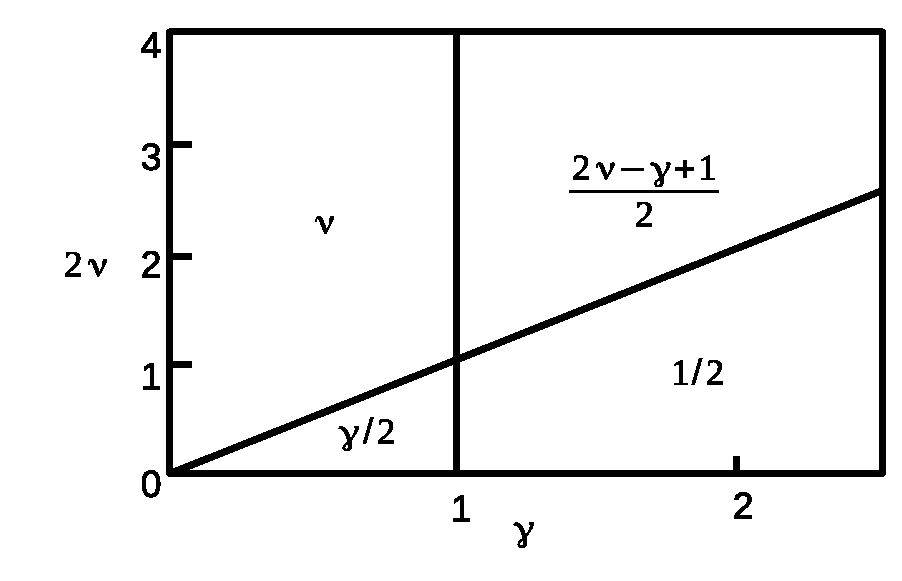
\includegraphics[width=90mm]{pics/alphaValuesPDF.eps}
\caption{Values of $\alpha$ in the different regions of parameter space. Solid lines correspond to changes in the regime.
\label{fig:alphaValuesPDF} }
\end{center}
\end{figure} 
%
There is no known solution for the inverse Laplace transform of this expression for general values of $\alpha$. However for the special case of $\alpha = \frac{1}{2} $ the result is known to be
%
\begin{align}
\gls{pdf}_{\alpha=1/2}(x|t) = \frac{1}{\sqrt{\pi}t}e^{-\frac{1}{4t}\abs{x}^2} ,
\end{align}
%
i.e. a Gaussian distribution with variance $\sqrt{2t}$. 

For the very similar one-side alpha-stable L\'evy distributions, whose Laplace transform reads
%
\begin{align}
f(s) = e^{-s^{\alpha}},
\end{align}
%
there exists a closed expression for all rational $\alpha<1$ derived in \cite{penson2010}, 
where the result is expressed in generalized hypergeometric functions. This can be related to our case via the Riemann-Liouville fractional derivative of order $\alpha-1$ 
\cite{mathai2009}. 
Unfortunately I was not able to find a closed expression for this result that could be evaluated.\\
However the second factor $e^{-\abs{x}s^{\alpha}}$ is always slowly varying in the limit $s \to 0$, therefore the Tauberian theorem in Eq. (\ref{eqn:tauberian}) tells us that the leading order of the inverse Laplace transformation will be proportional to $t^{-\alpha}$. While this loses the exact dependence on $\abs{x}$ it does predict how the \gls{PDF} will scale at the origin $\abs{x}=0$, which can be compared to the results of the simulation.

We can furthermore evaluate the inverse transform numerically using the powerful algorithm developed by Talbot 
\cite{talbot1979}, 
which I mentioned earlier. The results of this are presented in Sec. \ref{analyticResultsPDF}.